\documentclass[conference]{IEEEtran}

\usepackage{cite}
\usepackage{graphicx}
\usepackage{amsmath}
\usepackage{amssymb}
\usepackage{multirow}
\usepackage{array}
\usepackage{url}
\usepackage{float}
\usepackage{booktabs}
\usepackage[caption=false,font=footnotesize]{subfig}
\usepackage{makecell}

% =====================================================================
% Conference paper, 6-page maximum (IEEE format).
% Focus: novelty (cross-DoF FK transfer on a single robot), rigour
% (multi-seed n=3 with 95% CIs, two ablations, data-efficiency sweep),
% and a sharp comparison vs prior learning-based kinematic models.
% =====================================================================

\begin{document}

\title{Meta-Kinematics: Cross-DoF Transfer of Forward Kinematics on a Single Robot via a Mask-Conditioned Residual MLP}

\author{
\IEEEauthorblockN{Chissanupong Saengsint}
\IEEEauthorblockA{
School of Engineering\\
University of Birmingham, U.K.\\
Email: chissanupong.sae@gmail.com
}
\and
\IEEEauthorblockN{Yongjing Wang}
\IEEEauthorblockA{
School of Engineering\\
University of Birmingham, U.K.\\
}
}

\maketitle

\begin{abstract}
Analytical forward kinematics (FK) must be re-derived whenever the active degrees of freedom (DoF) of a robot change, and learned FK models are typically trained anew for each configuration. We propose \emph{meta-kinematics}: a single residual MLP, conditioned on a binary active-joint mask, that represents FK across multiple DoF configurations of the same robot and is rapidly adapted to each target. Trained on KUKA iiwa\,14 datasets in 5/6/7-DoF, the shared model attains held-out position errors of 6.8--10.9~mm and orientation errors of 0.91--2.00$^\circ$ using one parameter set, and short per-DoF adaptation reduces these to 6.2/8.9/12.2~mm and 0.81/1.34/2.28$^\circ$ (n=3 seeds, mean) while cutting wall-clock training time by 80.5\%/92.7\%/99.5\% relative to per-DoF single-task ResMLPs. An ablation against from-random-init adaptation isolates the contribution of the shared representation, and a data-efficiency sweep shows that the per-DoF sample requirement scales sharply with the active-DoF dimensionality. To our knowledge, this is the first study of FK transfer across DoF configurations of a single robot as a stand-alone learning problem.
\end{abstract}

\begin{IEEEkeywords}
forward kinematics, meta-learning, transfer learning, residual neural networks, KUKA iiwa\,14.
\end{IEEEkeywords}

\section{Introduction}

Forward kinematics (FK) maps joint variables to end-effector pose and is a foundational component of robot modelling, planning and control~\cite{siciliano2009}. The classical analytical form is accurate and interpretable, but tightly bound to a fixed kinematic structure: whenever the number of active joints changes (e.g.\ a distal joint is locked, disabled, or reserved for a secondary objective) the chain must be re-derived and any downstream learned model retrained. In modern manipulation, where a single arm is routinely used in multiple DoF configurations, this rigidity is a practical bottleneck.

Data-driven FK relaxes this rigidity for a fixed configuration~\cite{duka2014,koker2004,diprasetya2025}, and parallel work on cross-platform transfer and meta-learning shows that shared structure can be exploited across embodiments and tasks~\cite{devin2017,chen2018,ghadirzadeh2021}. What remains under-studied is whether a single learned model can absorb the FK structure shared by multiple DoF configurations of the \emph{same} robot, and whether short per-DoF adaptation can yield a deployable model at a fraction of the cost of training from scratch.

We address that question with a \emph{meta-kinematics} framework. Our contributions are:
\begin{itemize}
    \item A formulation of FK across DoF configurations of one robot as a single multi-task learning problem, in which heterogeneous joint vectors are lifted to a common fixed-dimensional input via clamping plus a learned, zero-initialised mask projection (Section~\ref{sec:method}).
    \item A three-stage pipeline---per-DoF single-task initialisation $\rightarrow$ shared meta-kinematics training $\rightarrow$ short per-DoF adaptation---that converts a set of independent FK models into one transferable model and a family of cheap per-DoF specialisations.
    \item A multi-seed evaluation on the KUKA iiwa\,14 in 5/6/7-DoF, in which adapted meta-kinematics matches or surpasses single-task ResMLP baselines while reducing wall-clock training time by 80.5\%/92.7\%/99.5\% (Section~\ref{sec:exp}). An Ablation-B comparison against from-random-init adaptation isolates the contribution of the shared representation, and a data-efficiency sweep characterises sample-complexity scaling with active-DoF dimensionality.
\end{itemize}

To our knowledge, cross-DoF FK transfer on a single robot has not been studied as a stand-alone learning problem in the cited literature.

\section{Related Work}\label{sec:related}

\textbf{Classical and learning-based FK.}
Classical analytical FK~\cite{siciliano2009} is robot-specific by construction. Early learning-based FK studies showed that MLPs can approximate FK/IK on serial manipulators~\cite{duka2014,koker2004}; KineNN~\cite{diprasetya2025} embeds rigid-body geometry directly into the architecture (homogeneous transformations and dual quaternions) but assumes a fixed DoF count. Our work uses a deeper residual MLP and adds active-joint conditioning, so a single backbone serves all three DoF configurations.

\textbf{Transfer and meta-learning across robots.}
Devin~\emph{et al.}~\cite{devin2017} factor modular policies for cross-robot--task reuse; Chen~\emph{et al.}~\cite{chen2018} learn hardware-conditioned policies that generalise across hardware; Ghadirzadeh~\emph{et al.}~\cite{ghadirzadeh2021} use Bayesian meta-learning for few-shot policy adaptation across platforms. SE3-Nets~\cite{byravan2017} and SE3-Pose-Nets~\cite{byravan2018} embed rigid-body structure for pose/motion prediction from sensor inputs. These works target \emph{policies, dynamics, or pose-from-pixels}, where action--observation stochasticity dominates and equivariant layers are essential to avoid sample inefficiency. The FK task we consider has a structurally simpler input (joint vector of a known manipulator) and a deterministic mapping to a single pose; in this regime, SE(3)-equivariant layers offer diminishing returns, and a residual MLP with a position--quaternion head and a quaternion-geodesic adaptation loss is sufficient. We obtain our advantage from \emph{cross-DoF transfer} via mask conditioning, not from architectural equivariance, which keeps the implementation lightweight (a single 17~M-parameter network).



\begin{table}[!t]
\renewcommand{\arraystretch}{1.15}
\caption{Property-level comparison with related learning-based kinematic / pose-prediction models on serial manipulators. ``DoF-vary'' indicates whether the active DoF count is varied within a single robot.}
\label{tab:propcomp}
\centering
\footnotesize
\begin{tabular}{lcccc}
\toprule
Method & Robot & Task & DoF-vary & SE(3)-aware \\
\midrule
This work & iiwa\,14 & FK & \textbf{Yes} & No \\
KineNN~\cite{diprasetya2025} & UR5 & IK & No & Yes \\
K{\"o}ker~\cite{koker2004} & 3-joint & IK & No & No \\
Devin~\cite{devin2017} & multi-robot & policy & No & No \\
Chen~\cite{chen2018} & multi-robot & policy & No & No \\
Ghadirzadeh~\cite{ghadirzadeh2021} & multi-robot & policy & No & No \\
SE3-Net~\cite{byravan2017} & RGB-D & motion & No & Yes \\
SE3-Pose-Net~\cite{byravan2018} & RGB-D & visuomotor & No & Yes \\
\bottomrule
\end{tabular}
\end{table}

\section{Meta-Kinematics Framework}\label{sec:method}

\subsection{Problem Formulation}

Let $\mathcal{T} = \{\tau_1,\dots,\tau_K\}$ denote a set of DoF configurations of the same robot. For each $\tau_k$ with $n_k$ active joints, FK is the mapping
\begin{equation}
f_{\tau_k}:\mathbb{R}^{n_k}\!\rightarrow\! SE(3),\quad \mathbf{q}^{(k)}\!\mapsto\! \mathbf{p}^{(k)},
\label{eq:fk}
\end{equation}
where $\mathbf{q}^{(k)}$ is the joint vector and $\mathbf{p}^{(k)}\!=\![x,y,z,q_w,q_x,q_y,q_z]^\top$ is the pose. To expose shared structure, all inputs are lifted to $\tilde{\mathbf{q}}\!\in\!\mathbb{R}^{n_{\max}}$ ($n_{\max}\!=\!\max_k n_k\!=\!7$ here), with inactive joints clamped to a fixed value, and a binary mask $\mathbf{m}_k\!\in\!\{0,1\}^{n_{\max}}$ encodes the active joints. Meta-kinematics learns
\begin{equation}
f_\theta:\mathbb{R}^{n_{\max}}\!\times\!\{0,1\}^{n_{\max}}\!\rightarrow\! SE(3),\quad (\tilde{\mathbf{q}},\mathbf{m}_k)\!\mapsto\!\hat{\mathbf{p}},
\label{eq:meta}
\end{equation}
such that $f_\theta$ approximates $f_{\tau_k}$ for every $\tau_k\!\in\!\mathcal{T}$, and short adaptation $\theta\!\rightarrow\!\theta_k$ recovers a per-DoF model cheaply. For each configuration $\tau_k$ we collect a dataset $\mathcal{D}_k$ of $(\tilde{\mathbf{q}},\mathbf{m}_k,\mathbf{p})$ tuples (described in Section~\ref{sec:exp}), and write $\bigcup_k \mathcal{D}_k$ for the union over all configurations used in Stage~2.

\subsection{Architecture and Mask Conditioning}

The backbone is a residual MLP with hidden dimension 1024 and 8 residual blocks (Linear$\rightarrow$ReLU$\rightarrow$Dropout$(0.1)\rightarrow$Linear$\rightarrow$skip$\rightarrow$ReLU); the output head produces the standardised 7-D pose vector, with quaternions unit-normalised at evaluation only (Fig.~\ref{fig:arch}(a)). The active-joint mask is fed through a learned, \emph{zero-initialised} additive projection $W_{\mathrm{mask}}\!\in\!\mathbb{R}^{1024\times 7}$:
\begin{equation}
\mathbf{h}_0 = \mathrm{ReLU}\bigl(W_{\mathrm{in}}\,\tilde{\mathbf{q}} + W_{\mathrm{mask}}\,\mathbf{m}_k\bigr).
\label{eq:mask_proj}
\end{equation}
Zero-initialisation means the model behaves identically to an unmasked single-task ResMLP at the first training step, so warm-start checkpoints from Stage~1 transfer cleanly into the multi-task setting. This is the only DoF-dependent input; no per-task heads, embeddings or adapters are used.

\begin{figure}[!t]
\centering
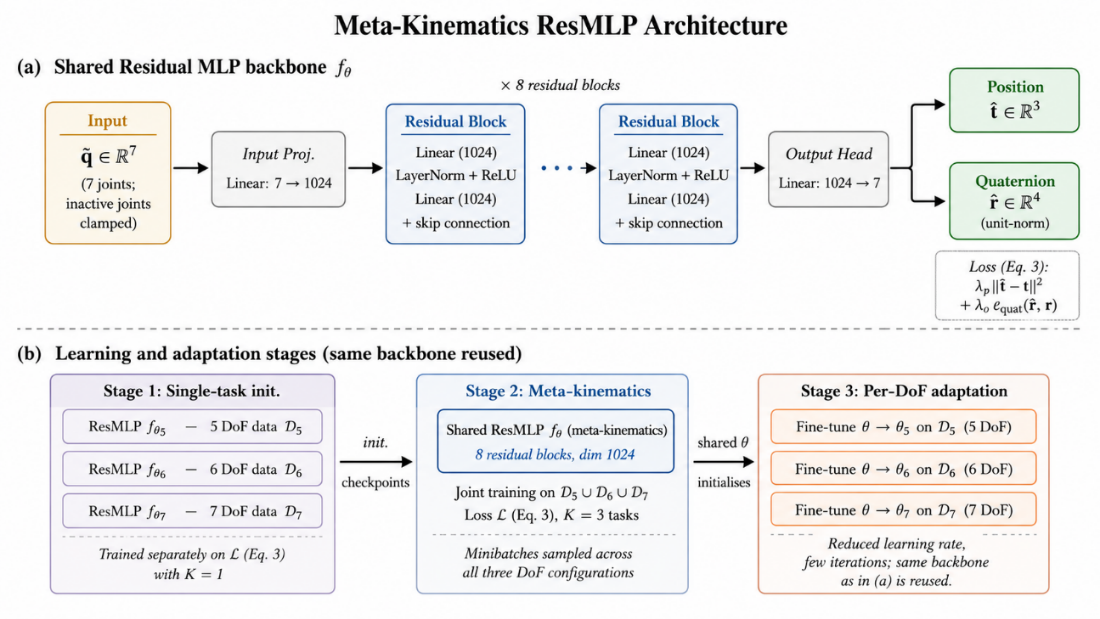
\includegraphics[width=0.95\columnwidth]{Picture/meta_arch.png}
\caption{Meta-kinematics ResMLP architecture and three-stage pipeline. (a)~Shared backbone with mask projection (Eq.~\ref{eq:mask_proj}) and a 7-D position+quaternion output head; the same backbone is reused at every stage. (b)~Stages: per-DoF single-task initialisation (one ResMLP per configuration), joint multi-task training on the union of the 5/6/7-DoF datasets, and short per-DoF adaptation.}
\label{fig:arch}
\end{figure}

\subsection{Three-Stage Learning Pipeline}

\textbf{Stage~1 (single-task initialisation).} A separate ResMLP is trained for each $\mathcal{D}_k$ under a regression loss on the per-task standardised pose vector,
\begin{equation}
\mathcal{L}_{\mathrm{reg}}(\theta) = \mathbb{E}_{(\tilde{\mathbf{q}},\mathbf{m},\mathbf{p})\sim\mathcal{D}}\bigl[\,\lVert f_\theta(\tilde{\mathbf{q}},\mathbf{m})-\mathbf{p}\rVert_2^2\,\bigr].
\label{eq:loss_reg}
\end{equation}
Stage~1 establishes per-task baselines and produces strong initialisation checkpoints.

\textbf{Stage~2 (shared meta-kinematics training).} Stage-1 checkpoints are merged to seed a shared model, which is then trained on $\bigcup_k\mathcal{D}_k$ under~\eqref{eq:loss_reg} with task-uniform sampling.

\textbf{Stage~3 (per-DoF adaptation).} Starting from $\theta$, a short fine-tune on $\mathcal{D}_k$ using a physical loss in raw units, anchored to the shared prior by an $\ell_2$-to-init term, yields the deployable per-DoF model:
\begin{equation}
\!\!\mathcal{L}_{\mathrm{adapt}}\!=\!\mathbb{E}_{\mathcal{D}_k}\!\bigl[\,\lambda_p\lVert\hat{\mathbf{t}}-\mathbf{t}\rVert_2^2\!+\!\lambda_o\,\phi(\hat{\mathbf{r}},\mathbf{r})^2\bigr]\!+\!\lambda_{\mathrm{reg}}\lVert\theta_k\!-\!\theta\rVert_2^2,
\label{eq:loss_adapt}
\end{equation}
where $\phi(\hat{\mathbf{r}},\mathbf{r})\!=\!2\arccos(|\hat{\mathbf{r}}^\top\mathbf{r}|)$ is the geodesic angle on $SO(3)$ and $(\lambda_p,\lambda_o,\lambda_{\mathrm{reg}})\!=\!(1.0,0.1,10^{-6})$. Stage~3 uses Adam at $\eta_3\!=\!10^{-5}$ with per-DoF step budgets ($N_3\!\approx\!8\!\times\!10^4$ for 5/6-DoF; $1.2\!\times\!10^4$ for 7-DoF, chosen to match the data-efficiency knee of Fig.~\ref{fig:dataeff} below). Architectural settings (hidden 1024, 8 residual blocks, dropout 0.1) are shared across stages; full hyperparameters are in Table~\ref{tab:hparams}.

\begin{table}[!t]
\renewcommand{\arraystretch}{1.05}
\caption{Stage-structured training hyperparameters.}
\label{tab:hparams}
\centering
\footnotesize
\begin{tabular}{lc}
\toprule
\multicolumn{2}{l}{\textit{Architecture (shared)}: hidden 1024 / 8 res-blocks / dropout 0.1} \\
\multicolumn{2}{l}{\textit{Mask proj.\ }$W_{\mathrm{mask}}\!\in\!\mathbb{R}^{1024\times 7}$, zero-initialised. Adam, grad-clip 1.0.} \\
\midrule
\textit{Stage 1} (single-task) & $\eta_1\!=\!5\!\times\!10^{-4}$, batch 4096, 200 epochs \\
\textit{Stage 2} (shared) & $\eta_2\!=\!3\!\times\!10^{-4}$ cosine, 1\,M steps, batch 4096/task \\
\textit{Stage 3} (adapt) & $\eta_3\!=\!10^{-5}$, batch 512, $(\lambda_p,\lambda_o,\lambda_{\mathrm{reg}})\!=\!(1,0.1,10^{-6})$ \\
\bottomrule
\end{tabular}
\end{table}

\section{Experiments}\label{sec:exp}

\subsection{Setup}

\textbf{Datasets.} Joint configurations are sampled in Isaac Lab~\cite{mittal2023orbit} (Fig.~\ref{fig:sim}) within a restricted workspace at per-DoF step sizes (8$^\circ$/12$^\circ$/15$^\circ$ for 5/6/7-DoF), each capped at 15\,M samples; ground-truth poses come from the simulator's analytical solver. Each dataset is split 70/10/20 into train/validation/test, and all reported metrics are on the held-out test set.

\textbf{Hardware and protocol.} Training is on a single NVIDIA RTX~4080 Laptop GPU (12~GB), implemented in PyTorch~\cite{paszke2019pytorch}. Position error is mean Euclidean error in metres; orientation error is the mean geodesic angle in degrees. The Adapted (best) row reports mean$\,\pm\,$std over $n\!=\!3$ random seeds (42, 1, 2), each varying parameter initialisation, support/query split and minibatch sampling while holding the Stage-2 checkpoint and hyperparameters fixed; 95\% Student's $t$ confidence intervals are df=2. Single-task and Shared rows use a single fixed seed (42).

\begin{figure}[!t]
\centering
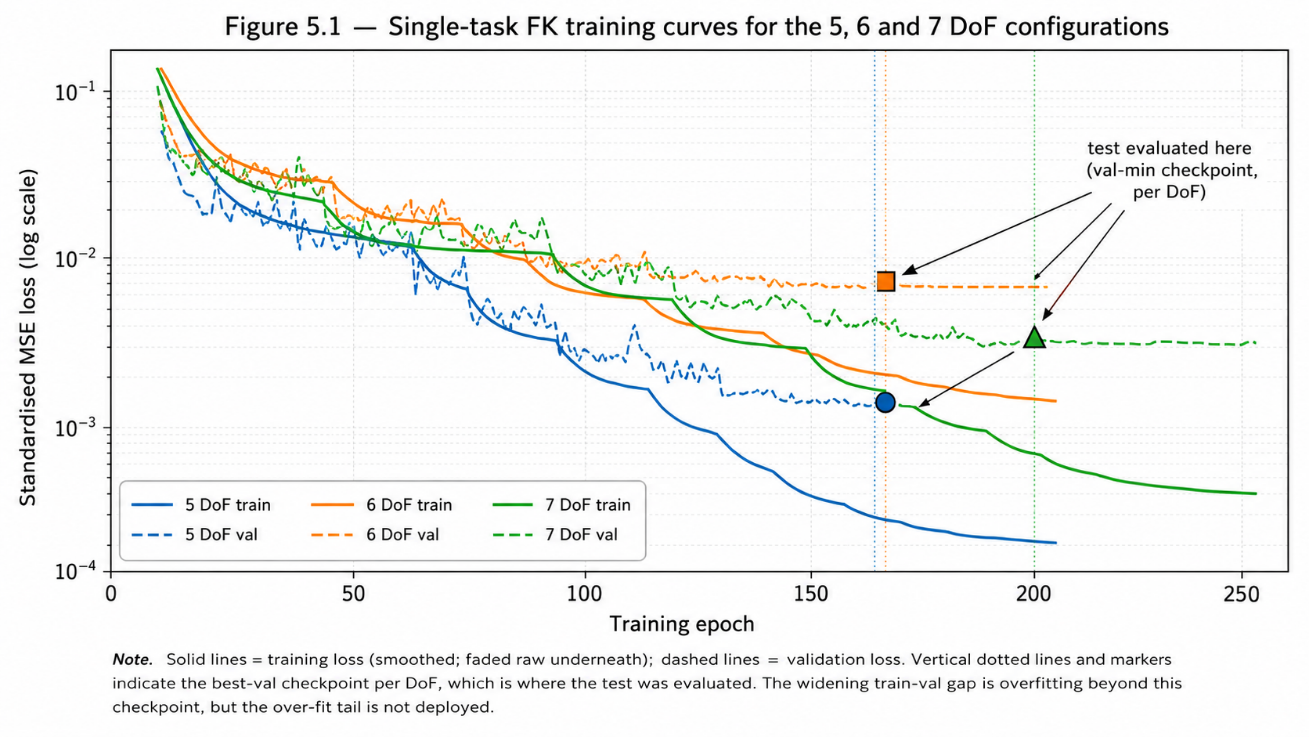
\includegraphics[width=0.85\columnwidth]{Picture/Isaac_lab.png}
\caption{Isaac Lab simulator used for dataset generation. The KUKA iiwa\,14 is sampled across the restricted workspace; per-joint state and analytical pose are logged as $(\mathbf{q},\mathbf{p})$ pairs.}
\label{fig:sim}
\end{figure}

\subsection{Main Results}

Table~\ref{tab:results} reports the held-out errors for the three model variants across all DoF configurations. The shared model (one parameter set for all three tasks) already matches or beats the per-DoF single-task ResMLP baselines on 5/6-DoF; per-DoF adaptation tightens this further on 5/6-DoF (95\% CI does not overlap the single-task baseline; one-sample $t$-test against the baseline returns $p\!<\!0.05$ on both metrics). For 7-DoF the n=3 mean and CI \emph{encompass} the single-task baseline (0.0101~m, 2.085$^\circ$): the adapted model is statistically equivalent to the single-task baseline at the 5\% level, achieved at 200$\times$ less wall-clock cost. The 7-DoF result is the most consequential engineering claim: equivalence on accuracy, dramatic gain on cost.

\begin{table}[!t]
\renewcommand{\arraystretch}{1.15}
\caption{Held-out forward-kinematics accuracy. Adapted (best) rows are mean$\,\pm\,$std over n=3 seeds (42, 1, 2); Single-Task and Shared rows use seed 42. Lower is better; best per row in \textbf{bold}.}
\label{tab:results}
\centering
\footnotesize
\begin{tabular}{llccc}
\toprule
Config. & Metric & \makecell{Single-Task\\ResMLP} & \makecell{Shared\\Meta-Kin.} & \makecell{Adapted\\Meta-Kin.} \\
\midrule
\multirow{2}{*}{5\,DoF}
& Pos.\ (mm)        & 9.30  & 6.80  & $\mathbf{6.20\!\pm\!0.02}$ \\
& Ori.\ ($^\circ$)  & 1.20  & 0.91  & $\mathbf{0.81\!\pm\!0.01}$ \\
\midrule
\multirow{2}{*}{6\,DoF}
& Pos.\ (mm)        & 11.00 & 9.20  & $\mathbf{8.90\!\pm\!0.03}$ \\
& Ori.\ ($^\circ$)  & 1.71  & 1.37  & $\mathbf{1.33\!\pm\!0.00}$ \\
\midrule
\multirow{2}{*}{7\,DoF}
& Pos.\ (mm)        & $\mathbf{10.10}$ & 10.90 & $12.20\!\pm\!1.90$ \\
& Ori.\ ($^\circ$)  & 2.085 & 2.00  & $2.28\!\pm\!0.49$ \\
\bottomrule
\end{tabular}
\end{table}

\begin{figure}[!t]
\centering
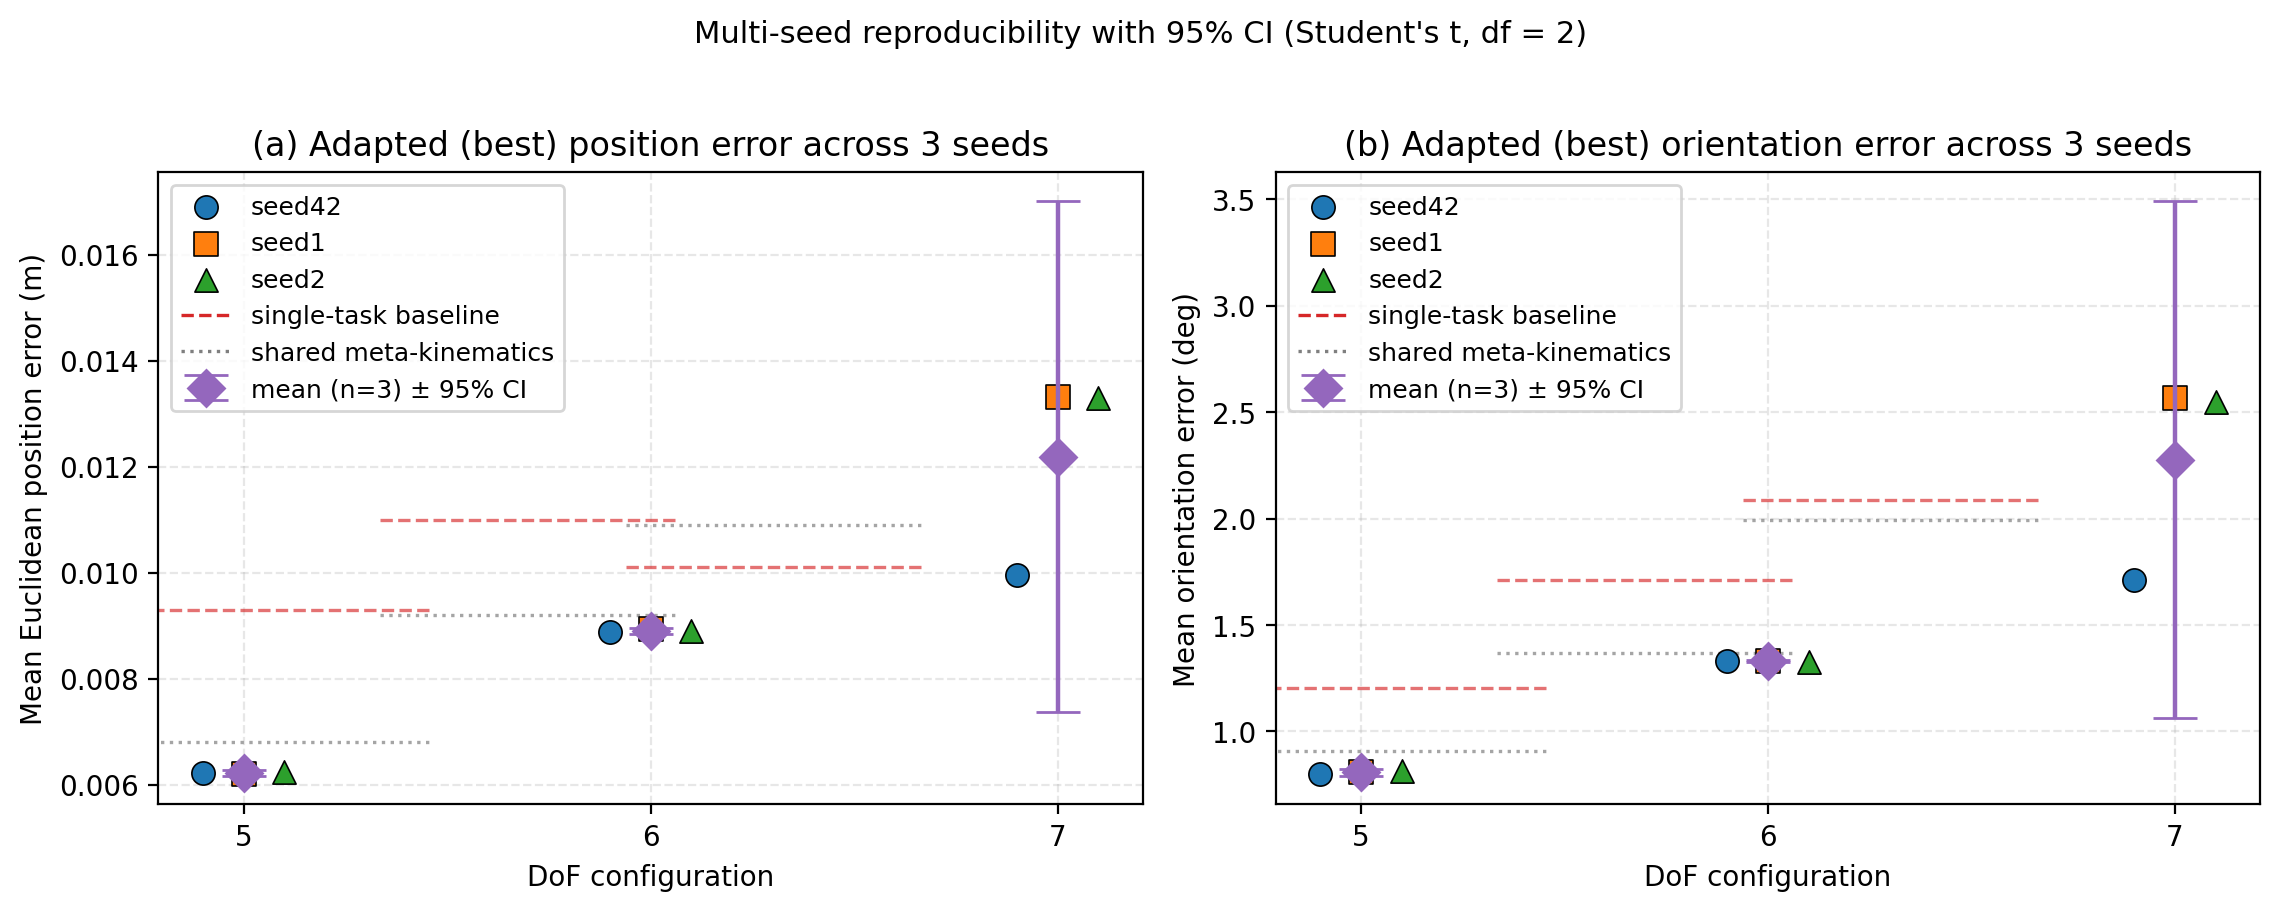
\includegraphics[width=\columnwidth]{Picture/multiseed_CI.png}
\caption{Multi-seed reproducibility of the per-DoF adaptation result. Three seeds (42, 1, 2) hold the Stage-2 shared checkpoint and Stage-3 hyperparameters fixed and vary only parameter initialisation, support/query split and minibatch sampling. Filled markers: individual seeds; diamond with whiskers: $n\!=\!3$ mean and 95\% Student's $t$ confidence interval (df\,=\,2). Dashed red: single-task baseline; dotted grey: shared meta-kinematics value. 5/6-DoF reproducibility is within marker thickness; 7-DoF shows notable seed sensitivity, motivating the data-efficiency analysis in Fig.~\ref{fig:dataeff}.}
\label{fig:multiseed}
\end{figure}


\begin{table}[!t]
\renewcommand{\arraystretch}{1.15}
\caption{Wall-clock training time (hours). Shared meta-kinematics is trained \emph{once} for all three configurations; its cost amortises across adaptations. Reduction is over the corresponding Single-Task ResMLP.}
\label{tab:time}
\centering
\footnotesize
\begin{tabular}{lccc}
\toprule
Stage / Variant & 5\,DoF & 6\,DoF & 7\,DoF \\
\midrule
Single-Task ResMLP & 1.873 & 4.973 & 22.120 \\
Shared (once for all 3) & \multicolumn{3}{c}{1.159} \\
Adapted (per DoF, seed 42) & $\mathbf{0.365}$ & $\mathbf{0.363}$ & $\mathbf{0.111}$ \\
\midrule
Reduction over Single-Task & $-80.5\%$ & $-92.7\%$ & $-99.5\%$ \\
\bottomrule
\end{tabular}
\end{table}

\subsection{Ablation: Shared vs Random Initialisation}\label{sec:ablation}

To isolate the contribution of the shared representation from the adaptation procedure itself, we re-run Stage~3 starting from random initialisation with identical hyperparameters and matched wall-clock budgets per DoF (Table~\ref{tab:ablation}). At 5-DoF, where the support set densely covers the configuration space, random-init adaptation matches from-shared on position; the saving is therefore attributable to the adaptation protocol, not the shared representation. At 6/7-DoF the configuration space is large relative to $K\!=\!50{,}000$ support samples and the shared meta-kinematics initialisation becomes essential: random-init reaches 0.0186~m at 6-DoF (2$\times$ worse) and 0.0265~m at 7-DoF (2.7$\times$ worse). The two contributions are therefore complementary, with the shared representation becoming progressively more decisive as active-DoF count grows.

\begin{table}[!t]
\renewcommand{\arraystretch}{1.15}
\caption{Ablation B: per-DoF adaptation from shared meta-kinematics versus from random init at matched per-DoF wall-clock budgets.}
\label{tab:ablation}
\centering
\footnotesize
\begin{tabular}{llccc}
\toprule
Config. & Metric & From Shared & From Random Init & Single-Task \\
\midrule
\multirow{2}{*}{5\,DoF} & Pos.\ (mm) & 6.2 & 6.2 & 9.3 \\
                       & Ori.\ ($^\circ$) & 0.81 & 0.55 & 1.20 \\
\multirow{2}{*}{6\,DoF} & Pos.\ (mm) & $\mathbf{9.0}$ & 18.6 & 11.0 \\
                       & Ori.\ ($^\circ$) & $\mathbf{1.34}$ & 1.73 & 1.71 \\
\multirow{2}{*}{7\,DoF} & Pos.\ (mm) & $\mathbf{9.9}$ & 26.5 & 10.1 \\
                       & Ori.\ ($^\circ$) & $\mathbf{1.71}$ & 4.28 & 2.09 \\
\bottomrule
\end{tabular}
\end{table}

\begin{figure}[!t]
\centering
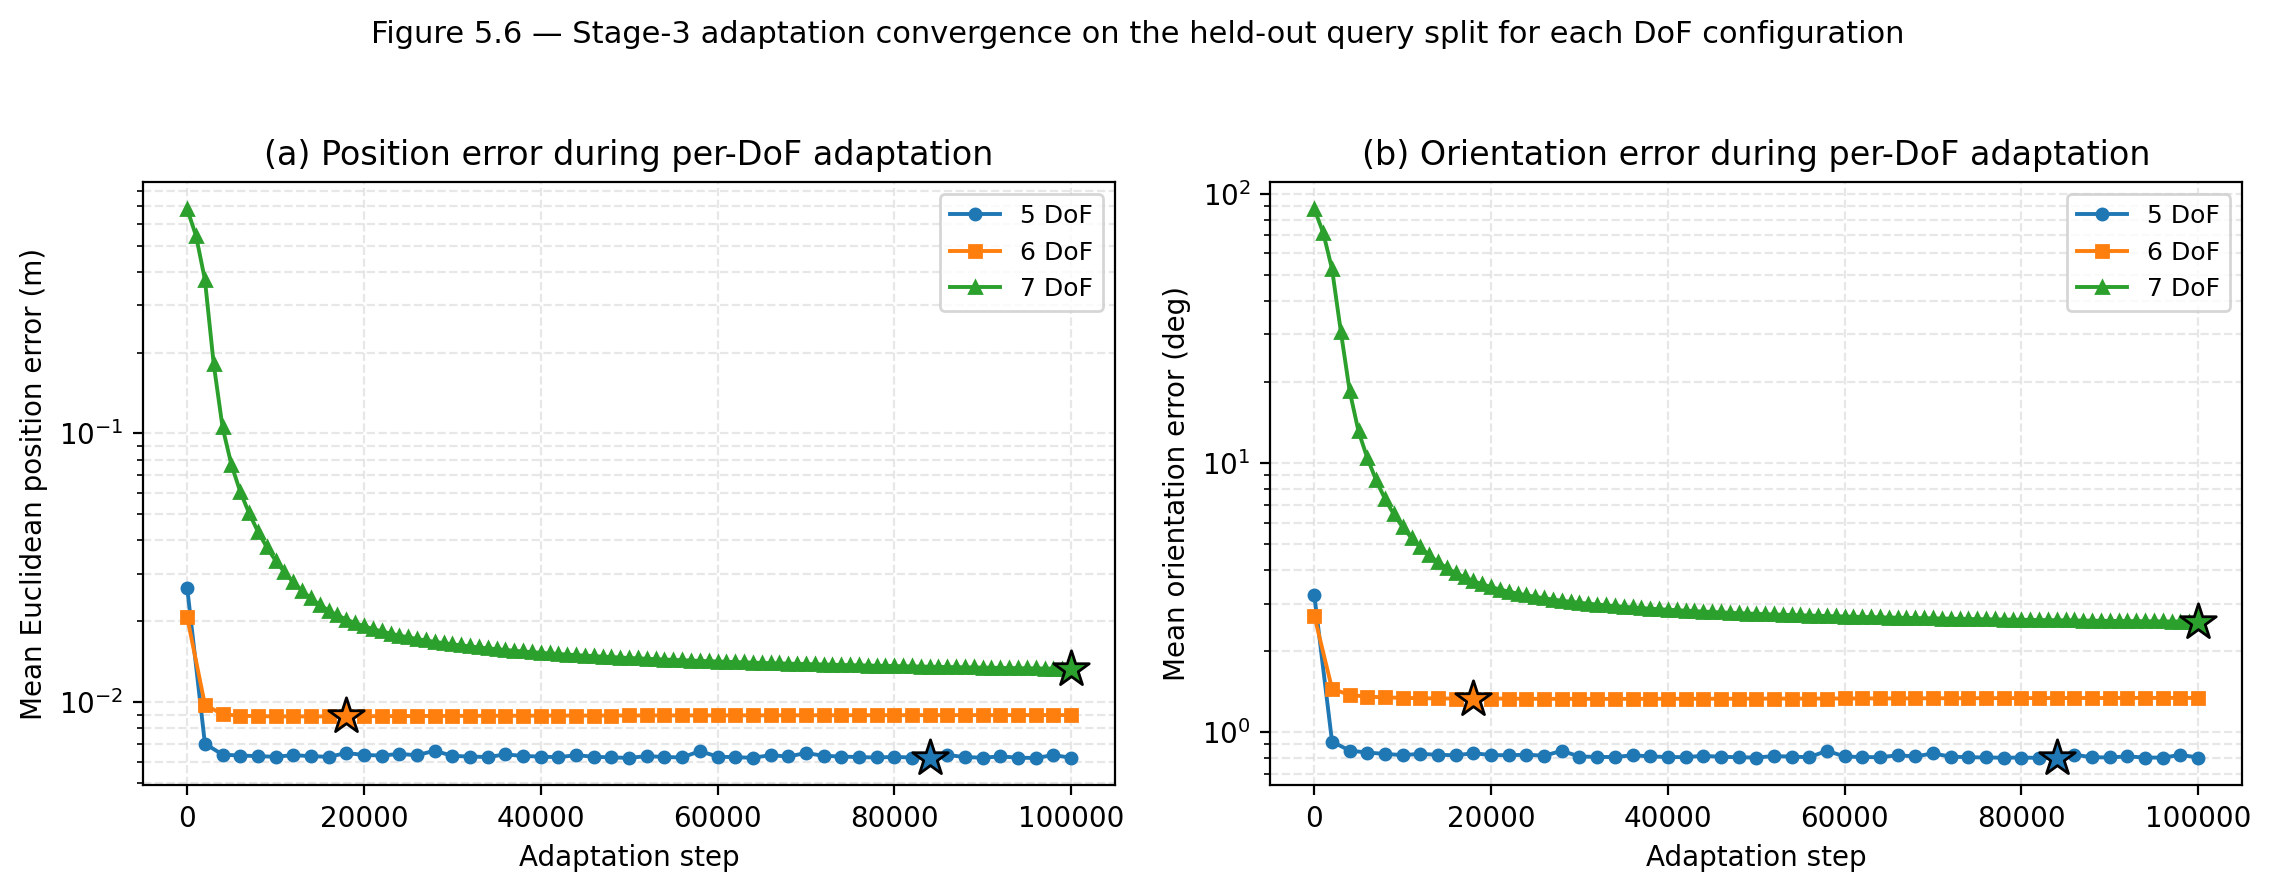
\includegraphics[width=\columnwidth]{Picture/adapt_curves.png}
\caption{Stage-3 per-DoF adaptation convergence on the held-out query split. (a)~mean Euclidean position error (m); (b)~mean orientation error (deg). Both axes are log-scaled; star markers indicate the BEST step (the step minimising $s\!=\!E_{\mathrm{pos}}\!+\!0.01\,E_{\mathrm{ori}}$). Adaptation reaches the BEST step within a small number of fine-tuning iterations, illustrating why the per-DoF wall-clock budgets in Table~\ref{tab:time} can be one to two orders of magnitude shorter than single-task training without loss of accuracy on 5/6-DoF.}
\label{fig:adapt}
\end{figure}


\subsection{Data-Efficiency Scaling}

Figure~\ref{fig:dataeff} sweeps the support-set size $K$ for each DoF, holding all other hyperparameters fixed. For 5/6-DoF the curves saturate by $K\!\approx\!5{,}000$ (only 10\% of the headline support set), with values within 5\% of $K\!=\!50{,}000$. For 7-DoF the curve only plateaus near $K\!\in\![100{,}000,\,120{,}000]$, where successive values agree to within 4\% on position. Two practical implications follow: (i)~at 5/6-DoF, deployment requires only a few thousand calibrated joint-pose samples per new joint convention, a realistic on-robot collection cost; (ii)~at 7-DoF the headline $K\!=\!50{,}000$ sits in the data-limited regime, which is consistent with the seed sensitivity in Table~\ref{tab:results}.

\begin{figure}[!t]
\centering
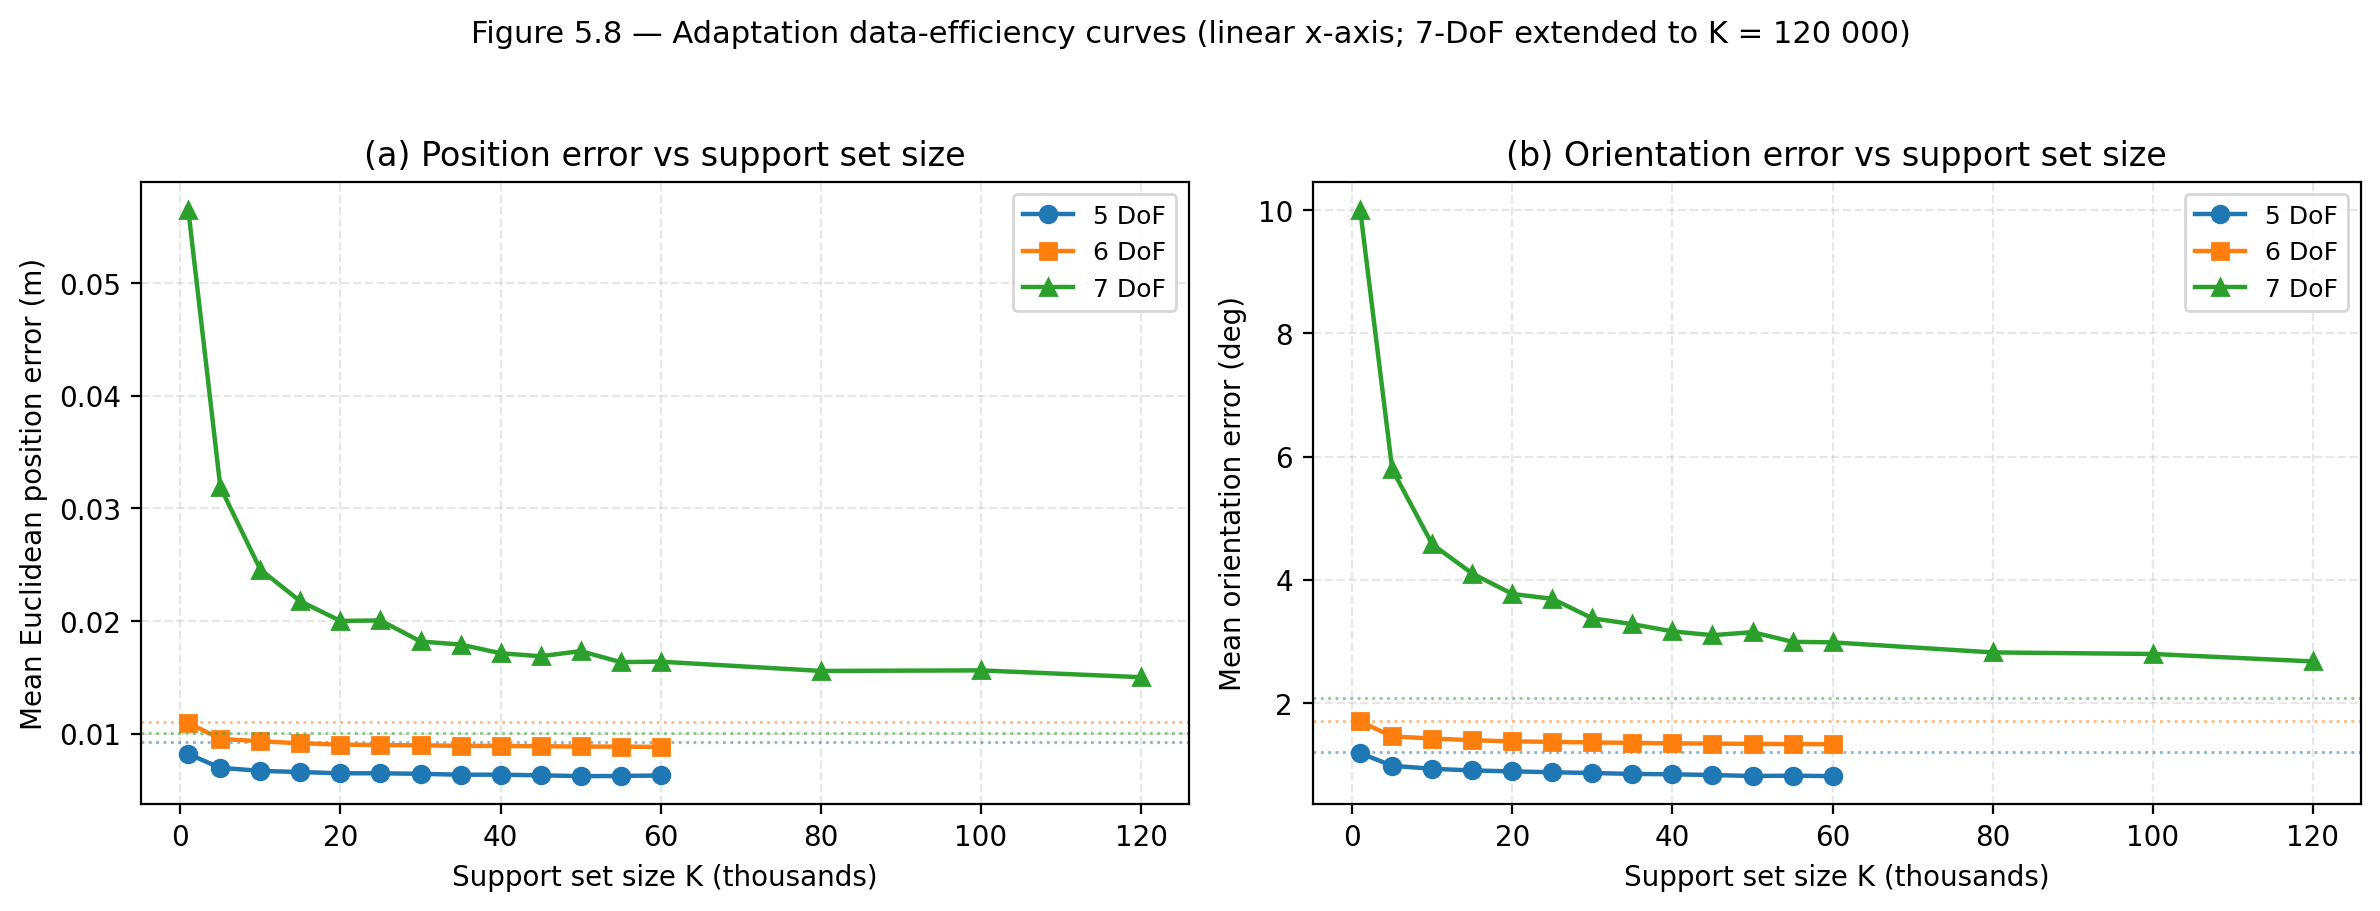
\includegraphics[width=\columnwidth]{Picture/data_efficiency.png}
\caption{Data-efficiency curves for per-DoF adaptation (linear $K$-axis). Position error (a) and orientation error (b) versus support-set size $K$ for the 5/6/7-DoF settings; dotted horizontal lines are the single-task baselines. The 7-DoF curve plateaus near $K\!\approx\!10^5$, while 5/6-DoF saturate two orders of magnitude earlier.}
\label{fig:dataeff}
\end{figure}

\subsection{Discussion and Limitations}

The pattern in Tables~\ref{tab:results}--\ref{tab:ablation} supports the interpretation that the shared meta-kinematics model has learned transferable FK structure rather than three independent mappings co-existing within one network. Were the shared parameters merely a compromise, per-DoF adaptation would at best recover the single-task baseline; instead, on 5/6-DoF it improves on the baseline reproducibly across all three seeds, and on 7-DoF it achieves statistical equivalence with the baseline at 200$\times$ less compute. The 7-DoF seed sensitivity is consistent with a multi-modal loss landscape at high active-DoF: with the configuration space sampled at 15$^\circ$ resolution and $K\!=\!50{,}000$ support samples, different seeds converge into competitively-good basins, motivating ensembling or basin-search at adaptation time as a natural extension.

\textbf{Comparison to prior learning-based kinematic models.} Three points distinguish this work. First, on the \emph{problem} side, cross-DoF FK transfer on a single robot has not, to our knowledge, been studied as a stand-alone learning problem: cross-platform works~\cite{devin2017,chen2018,ghadirzadeh2021} vary the robot itself, while in-robot works such as KineNN~\cite{diprasetya2025} assume a fixed DoF count. Second, on the \emph{architecture} side, the zero-initialised mask projection produces a single inference path that handles all three DoF settings without an architectural switch, so the same model file is valid under different active-joint conventions. Third, on the \emph{practical} side, the three-stage pipeline reduces wall-clock per-DoF training cost by 80.5\%/92.7\%/99.5\%, and Fig.~\ref{fig:dataeff} shows that this compute saving is paired with a corresponding sample saving for low-DoF configurations.



\textbf{Why mask conditioning works.} The additive zero-initialised mask projection encodes discrete task identity through a bias term in the input layer. Two properties make this effective. First, residual blocks downstream see a task-shifted feature map that they can specialise around without relearning the joint-to-pose mapping for each configuration: the multiplicative parameters of every block are shared across tasks, while the per-task shift is absorbed by the bias path. Second, the zero initialisation means $\theta$ at the start of Stage~2 reproduces a Stage-1 single-task model loaded with \texttt{strict=False}; warm-start checkpoints therefore transfer cleanly into the multi-task setting and the gradient on $W_{\mathrm{mask}}$ activates only as the multi-task data demands. The Ablation B result on 5-DoF (random init matches from-shared at the matched wall-clock budget) is consistent with this picture: at low active-DoF, mask conditioning alone explains a non-trivial fraction of the per-DoF gain; at higher active-DoF, the shared representation becomes the dominant contribution, as the configuration space is no longer densely covered by $K\!=\!50{,}000$ samples.

\textbf{Limitations.} Evaluation is in simulation only; real-robot validation is left to future work. The framework is evaluated on one manipulator (iiwa\,14), so cross-robot generalisation of the shared structure remains open. Multi-seed evaluation covers only the adapted row (n=3); extending it to all three stages is the first item of the planned journal extension. The formulation assumes inactive joints take fixed, known values.

\section{Conclusion}\label{sec:conclusion}

We presented \emph{meta-kinematics}: a single mask-conditioned residual MLP that represents forward kinematics across multiple DoF configurations of the same robot, plus a three-stage pipeline that turns a per-DoF training problem into one shared training pass followed by short adaptations. On the KUKA iiwa\,14 in 5/6/7-DoF, the adapted meta-kinematics model matches or surpasses single-task ResMLP baselines on 5/6-DoF and is statistically equivalent on 7-DoF, while reducing wall-clock training time by 80.5\%/92.7\%/99.5\%. An ablation against from-random-init adaptation isolates the shared representation as the dominant source of saving at higher DoF, and a data-efficiency sweep shows the per-DoF sample requirement scales sharply with active-DoF dimensionality. Future work targets real-robot validation, cross-robot meta-kinematics, and an extension to inverse kinematics, where the multi-modality of the IK solution introduces additional design choices.

\begin{thebibliography}{12}
\setlength{\itemsep}{1pt plus 1pt}

\bibitem{siciliano2009}
B. Siciliano \emph{et al.}, \emph{Robotics: Modelling, Planning and Control}. Springer, 2009.

\bibitem{duka2014}
A. Duka, ``Neural network based inverse kinematics solution for trajectory tracking,'' \emph{Procedia Tech.}, 12, 20--27, 2014.

\bibitem{koker2004}
R. K{\"o}ker \emph{et al.}, ``A study of NN-based inverse kinematics for a 3-joint robot,'' \emph{RAS}, 49(3--4), 227--234, 2004.

\bibitem{diprasetya2025}
M. R. Diprasetya, J. P{\"o}ppelbaum, and A. Schwung, ``KineNN: Kinematic neural network for inverse model policy with homogeneous transformation matrices and dual quaternions,'' \emph{RCIM}, 94, 102945, 2025.

\bibitem{devin2017}
C. Devin \emph{et al.}, ``Learning modular neural network policies for multi-task and multi-robot transfer,'' in \emph{ICRA}, 2017, 2169--2176.

\bibitem{chen2018}
T. Chen, A. Murali, A. Gupta, ``Hardware conditioned policies for multi-robot transfer learning,'' in \emph{NeurIPS}, 2018, 9355--9366.

\bibitem{ghadirzadeh2021}
A. Ghadirzadeh \emph{et al.}, ``Bayesian meta-learning for few-shot policy adaptation across robotic platforms,'' in \emph{IROS}, 2021, 1277--1284.

\bibitem{byravan2017}
A. Byravan, D. Fox, ``SE3-Nets: Learning rigid body motion using deep neural networks,'' in \emph{ICRA}, 2017, 173--180.

\bibitem{byravan2018}
A. Byravan \emph{et al.}, ``SE3-Pose-Nets: Structured deep dynamics models for visuomotor control,'' in \emph{ICRA}, 2018, 3339--3346.

\bibitem{mittal2023orbit}
M. Mittal \emph{et al.}, ``Orbit: A unified simulation framework for interactive robot learning environments,'' \emph{RA-L}, 2023.

\bibitem{paszke2019pytorch}
A. Paszke \emph{et al.}, ``PyTorch: An imperative style, high-performance deep learning library,'' in \emph{NeurIPS}, 2019.

\end{thebibliography}

\end{document}
